\documentclass[12pt]{jarticle}
% ページサイズの調整
\setlength{\oddsidemargin}{-0pt}
\setlength{\topmargin}{-20pt}
\setlength{\headheight}{-0pt}
\setlength{\headsep}{15pt}
\setlength{\textwidth}{16cm}
\setlength{\textheight}{23.5cm}
\setlength{\footskip}{70pt}

\usepackage[dvipdfmx]{graphicx,color}
\usepackage{multirow}
\renewcommand{\labelenumi}{(\theenumi)}

\usepackage{url}
\usepackage{enumitem}
\usepackage{booktabs}
\newcommand\doubleRule{\toprule\toprule}
\usepackage{subcaption}
\usepackage{pifont}
\usepackage[toc,page]{appendix}
\renewcommand{\appendixtocname}{付録}
\renewcommand{\appendixpagename}{付録}
\DeclareCaptionSubType * [alph]{table}
\captionsetup[subtable]{labelformat=simple, labelsep=space}
\renewcommand\thesubtable{\thetable(\alph{subtable})}
\usepackage{pgfplots}


\begin{document}

%------------%
%    表紙    %
%------------%
\thispagestyle{empty}
\begin{center}
\vspace*{1zw}
{\Large 平成29年度 卒業研究報告書} \\
\vspace*{7zw}
{\LARGE 機械学習による} \\
\vspace*{0.5zw}
{\LARGE 難読化されたプログラムのステルス評価} \\
\vspace*{20zw}
%{\large 提出日:\和暦\today} \\
{\large 提出日:\today} \\
\vspace*{5zw}
{\large 熊本高等専門学校 人間情報システム工学科} \\
\vspace*{2zw}
{\LARGE バラタ} \\
\vspace*{6zw}
{\large 指導教員:神崎 雄一郎 (准教授)}
\end{center}

%------------%
%    内容    %
%------------%

%\setcounter{tocdepth}{3}
\tableofcontents % 目次の出力

\newpage

\section{はじめに}  \label{sec:introduction}
商用のソフトウエアは,ライセンスキーや商業的価値のあるアルゴリズムなどのユーザに知られたくない秘密情報を含む場合がある.悪意のあるエンドユーザが物理的にソフトウエアを所有した場合,逆アセンブラやデバッガなどを用いて内部のコードを解析すればこのような秘密情報が取得される可能性がある.このような攻撃はman-at-the-end (MATE)攻撃と呼ばれ,MATE攻撃からソフトウエアを保護するために,難読化が広く用いられている.難読化は,ソフトウエアの機能を保持しながら,内部のコードを変形し,解析を困難にする.

難読化手法の品質は,人間の攻撃者に対する解析しにくさ「効力」(\textit{potency}),自動解析に対する耐性「耐性」(\textit{resilience}),変形による性能変化の度合「コスト」(\textit{cost}),保護されていないコードとの区別のつきにくさ「ステルス」(\textit{stealth})といった4つの項目によって評価を行うことが考えられる~\cite{resilience-banescu}.本研究では難読化されたプログラムのステルスに着目する.難読化によって変形されたコードがめずらしい特徴を持つことで目立つ,つまり,ステルスが低くなる場合,難読化によって保護されている秘密情報の場所が攻撃者に知られやすくなり,難読化の効果の低下につながる.そのため,難読化されたプログラムのステルスを評価する方法は重要である.

本研究では,ステルスを評価する方法の1つとして,コードの不自然さ(\textit{artificiality})を数値化する方法~\cite{code-art}および機械学習の手法を組み合わせて,あるプログラムが難読化されているかを判定するフレームワークを提案する.このフレームワークを用いて,与えられたプログラムが難読化されているかを判定するモデルを構築してケーススタディを行い,次のリサーチ・クエスチョンについて考察する.

\begin{description}
  \item[Q1]難読化された・されていないプログラムは分類・検出できるか?
  \item[Q2]特徴が強い難読化方法があるか?
\end{description}


\newpage

\section{アプローチ} \label{sec:approach}
与えられたプログラムが難読化されているかを判定するモデルを構築するためのフレームワークを図~\ref{fig:framework}に示す.この図では,使用したツールの入出力(プログラムやデータ)を楕円で,使用したツールを四角形で表す.フレームワークの流れとしては,まず難読化されていないプログラム(ノーマルプログラム)を用意して,難読化ツールによってコードの変形を行う(Step 1).得られた難読化されたプログラムと,ノーマルプログラムをプログラムの特徴を取り出すツールに与えて,機械学習のための学習データを取得する(Step 2).本研究では,逆アセンブラであるIDA\footnote{IDA: \url{https://www.hex-rays.com/products/ida/}}や確率的言語モデルを構築するSRILM\footnote{SRILM: \url{http://www.speech.sri.com/projects/srilm/}}といったツールに加えて,コードの不自然さ~\cite{code-art}の数値化方法を用いてプログラムの特徴を取得する.最後のステップ(Step 3)では,機械学習のアルゴリズムを使用して判定モデルを構築し,モデルの有効性を評価する.

一定のルールに従ってコード変形方法を用いた以上,各難読化手法には,論理的に何らかの判定できる特徴を生成すると考えられる~\cite{pinpoint}.したがって,機械学習によってデータを分類したり,データに含まれる外れ値を検出したり可能性があると考える.

機械学習の分類手法は,教師あり学習,つまり,既知のデータ(訓練データ) にクラスラベルを付けてモデルを学習し,未知のデータや将来のデータを予測する.異常検知手法は,ラベルは用いずに,多数のデータの中から異常なデータを検出する.本研究では,これらの方法を応用して,与えられたコードを「難読化されたコード」と「難読化されてないコード」に分類させたり,与えられたコードが「異常」かどうかを判定させたりする実験を行い,得られた結果から難読化されたコードのステルス(コードの目立ちにくさ)の評価を行う.

\begin{figure}[hb]
 \centering
 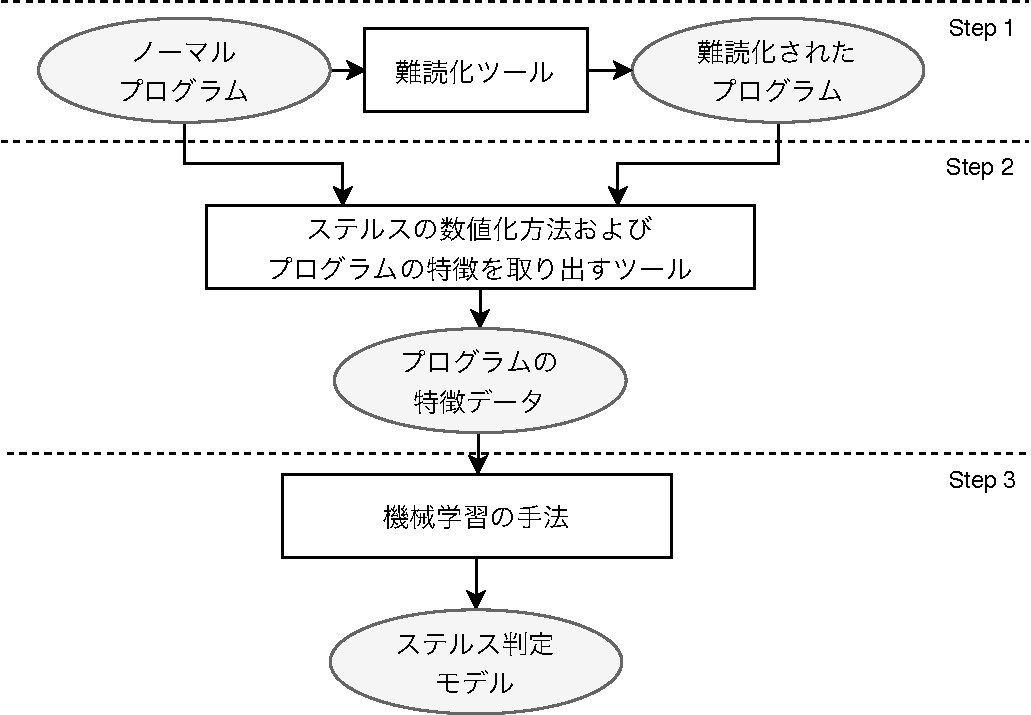
\includegraphics[width=12cm]{framework.pdf}
 \caption{提案フレームワークの概要}
 \label{fig:framework}
\end{figure}

\newpage

\section{ケーススタディ} \label{sec:casestudy}
本章では,~\ref{sec:approach}章で提案されたフレームワークに沿って,実際に判定モデルを構築し,リサーチ・クエスチョンについて調べる.

\subsection{ノーマルプログラム}
Step 1に記述されたノーマルプログラムとしては,様々な特徴を持つ多くのプログラムを収集することが望ましい.しかし,オープンソースのプログラムは保護したいコードを含むとは限らない上,難読化後の動作確認が難しい場合がある.このため,CentOS\footnote{CentOS: \url{https://www.centos.org/}}のシステムに分類される多様な460個のプログラム集合$P_{centos}$に加えて,Tigress~\cite{tigress}の\texttt{RandomFuns}変形オプションを使用して,難読化後の動作確認がしやすく,かつ,保護すべきコードを含むプログラムを数多く生成する.実験では,Tigressによってプログラムを288個生成された.\texttt{RandomFuns}機能は関数単位で動作し,生成された関数はライセンスチェックのようなルーチンであり,難読化の目的はこの機構を保護することである.本実験で調整した\texttt{RandomFuns}のパラメータの説明を付録~\ref{appendix:randfuns}に示す.この288個のプログラム集合$P_{orig}$は,実行時にコマンドラインから4つの引数「\texttt{42 42 42 42}」,パスワード「\texttt{secret}」を与えれば,``You win!''というメッセージが標準出力される.

\texttt{RandomFuns}によって生成されたプログラムは特徴を持つ可能性があり,多様性を高めるためにTigressの\texttt{split}オプションを用いて,$P_{orig}$の各プログラムにある1つの関数を複数の独立した関数に分割するコード変形を適用した.これらの288個のプログラム集合を$P_{split}$と表記する.

\subsection{難読化手法}
対象プログラムが多いことや実験の再現性を考慮した上で,難読化ツールを使用してコード変形を行う.コード変形の対象は\texttt{RandomFuns}により生成された288個のプログラム($P_{orig}$)であり,行ったコード変形の概要を次に示す.

\begin{enumerate}[leftmargin=*]
  \item$P_{aaa}$: 関数呼び出しの難読化が適用されたプログラム \\
  ある関数への呼び出しを理解しにくい間接的な呼び出し方法に書き換える難読化法が適用されたプログラムである.
  \item$P_{addop}$: 理解しにくい条件分岐を挿入する難読化が適用されたプログラム \\
  理解しにくく,かつ,どのような入力に対しても常に真か偽を返すような条件分岐を元のコードに挿入する難読化法が適用されたプログラムである.本実験では,10個の条件分岐を挿入した.
  \item$P_{enca}$: 整数の算術の難読化が適用されたプログラム \\
  算術の式をより複雑な式に書き換える難読化方法が適用されたプログラムである.
  \item$P_{encl}$: 整数と文字列リテラルの難読化が適用されたプログラム \\
  静的な整数または文字列のリテラルを,動的に同じ値を出力する関数に書き換える難読化法が適用されたプログラムである.
  \item$P_{flat}$: 制御フローの平滑化が適用されたプログラム \\
  ループや条件文のネストなどの制御構造を平滑化する難読化法が適用されたプログラムである.
  \item$P_{vir}$: インタプリタエンジンを用いた難読化が適用されたプログラム \\
  全てのコードを独自のバイトコードに書き換え,そのバイトコードを解釈するためのインタプリタを挿入する難読化法が適用されたプログラムである.
  \item$P_{jmp}$: 分岐命令のカムフラージュが適用されたプログラム \\
  文献~\cite{jmp-obf}で提案されたプログラムに含まれる分岐命令を非分岐命令でカムフラージュする動的な難読化方法が適用されたプログラムである.
\end{enumerate}
上記の(1)から(6)までの変形はTigressにより,(7)の$P_{jmp}$は文献~\cite{jmp-obf}の方法で試作したツールにより行った.コード変形後,動作確認を行い,$288\times7=2,016$個の全てのプログラムが正常に動作していると確認した.これでStep1が完了した.

\subsection{メトリクス} \label{sub:metrics}
Step 2では訓練データの特徴を取得し,本研究のステルス評価に使用された特徴量をこの章に説明する.また,本研究の確率的言語モデルにおける基本構成要素であるコードにある2レベルの粒度(\textit{granularity})についても説明する.

\begin{table}[!b]
\centering
\caption{評価対象プログラムのリスト}
\label{table:proglist}
\begin{tabular}[t]{c|c|l}
\doubleRule
\textbf{プログラム集合の名称} & \textbf{関数の数} & \multicolumn{1}{c}{\textbf{適用された難読化}}\\
\hline
$P_{centos}$ & 28,469 & なし(CentOSのシステムプログラム) \\
$P_{orig}$ & 2,592 & なし(\texttt{RandFuns}によって生成されたもの) \\
$P_{split}$ & 5,760 & なし(関数の分割を適用したもの) \\\hline
$P_{aaa}$ & 2,880 (576) & 関数呼び出しの難読化 \\
$P_{addop}$ & 2,880 (570) & 理解しにくい条件分岐を挿入する難読化 \\
$P_{enca}$ & 2,880 (576) & 整数の算術の難読化 \\
$P_{encl}$ & 4,896 (576) & 整数と文字列リテラルの難読化 \\
$P_{flat}$ & 2,880 (576) & 制御フローの平滑化 \\
$P_{vir}$ & 2,880 (576) & インタプリタエンジンを用いた難読化 \\
$P_{jmp}$ & (2,304) & 分岐命令のカムフラージュ \\
\bottomrule
\end{tabular}
\end{table}

実験上では,CentOSのプログラムに含まれるアセンブリコードをコーパスとして使用している.\texttt{mov, push}のような単純なコードと,\texttt{mov\_r.CODE, mov\_w.BSS}のような命令の書き込み「\texttt{\_w}」または読み込み「\texttt{\_r}」操作や操作する際に参照されるアドレスのセグメント(\texttt{CODE, BSS})の詳細な情報を含むコードの2種類の3-gramモデルのコーパスを使用した.本論文では,前者を「OPC」,後者を「XRF」で表記し,これらはコードの粒度という.

Tigressによるコード変形は関数単位で適用されるめ,3.1と3.2章に準備した$460+288+2,304=3,052$個のプログラムも関数単位で評価し,各プログラムグループの名称,合計の関数の数,適用されたコード変形や取得方法の概要を表~\ref{table:proglist}に示す.括弧で囲まれる関数の数は難読化された関数の数を示している.これらのプログラムをIDAで逆アセンブリし,以下の学習メトリクスを求める.

\begin{enumerate}
  \item \textbf{Art}: 関数を構成するコード全体の不自然さの指標である.コードの不自然さについては付録~\ref{appendix:artAndsurp}に示す.
  \item \textbf{Max}: コードを3-gram分割したときの関数の最大の「驚き値」(付録~\ref{appendix:artAndsurp})である.関数内の最も目立つコード列を見つけ出すという目的を持つメトリクスである.
  \item \textbf{OT}: 3-gramのコード片の驚き値を求め,定められた閾値を超えた関数内のコード片の数である.閾値は,$P_{centos}$のMaxの平均値から求められ,OPCを7.42,XRFを7.77に設定した.つまり,あるコード片の驚き値が,多様な難読化されていないプログラムのMaxの平均値を超えた場合,そのコード片が異常であると考えられ,異常なコード片の総数を示すメトリクスである.
  \item \textbf{Len}: 関数に含まれるコードの総数である.
  \item \textbf{Unq}: 関数内の独特なコードの数である.例えば,関数が5つの\texttt{mov, and, push, push, mov}のコード$I=i_1...i_5$から構成されているとき,$i_n\in$ \{\texttt{mov, and, push}\}であり,$|i_n|=3$であるから,Unqは3となる.また,XRFの場合,\texttt{mov\_r.CODE, mov\_w.BSS}はいずれも\texttt{mov}命令であるが,命令操作や参照されるアドレスセグメントが異なるため,2つの独特なコードとして扱うことにしている.このメトリクスは,例えば\texttt{mov}のみを生成するコンパイラ~\cite{movfuscator}によって生成されるコードの特徴を把握できる.
\end{enumerate}
(1)から(3)までのメトリクスは逆アセンブリされたプログラムのコードとコーパスをSRILMに与えて求めた.

\subsection{機械学習モデル}
Step 3の実行に当たって,まず,データの特徴を把握するために,各メトリクス間の線形な関係の強弱指標である相関係数を求める必要がある.表~\ref{table:correl}は,全てのデータを結合した後のピアソン相関係数~\cite{pearson}を示し,全ての係数は正であることから全てのメトリクス間は比例することが分かる.

\begin{table}[th]
\centering
\caption{各メトリクスの相関係数}
\label{table:correl}
\begin{tabular}[t]{c|ccccc}
\doubleRule
& Art & Max & Unq & Len & OT \\
\hline
Art & 1.0  & 0.30 & 0.46 & 0.96 & 0.73 \\
Max & 0.30 & 1.0  & 0.44 & 0.28 & 0.31 \\
Unq & 0.46 & 0.44 & 1.0  & 0.52 & 0.27 \\
Len & 0.96 & 0.28 & 0.52 & 1.0  & 0.57 \\
OT  & 0.73 & 0.31 & 0.27 & 0.57 & 1.0  \\
\bottomrule
\end{tabular}
\end{table}

最大の相関係数はArtとLenの間の0.96であり,この2つのメトリクスは非常に強く関係し,関数に含まれるコードが多いほど関数が不自然であると解釈できる.次に大きい相関係数はArtとOTの間の0.73であり,閾値を超えたコード片の数が多いほど関数が不自然であるといえる.UnqとOT以外の他のメトリクスや,OTとLenが[0.4, 0.6)の範囲にあることから,独特なコード数が多いほどコード全体が不自然になるとは限らず,関数が長いほど独特なコード数や閾値を超えたコード片の数も増えるとは限らない.残りの係数は[0.2, 0.4)の範囲に存在し,これらのメトリクスの間は弱く関係すると考えられる.

モデルを構築するためにPython\footnote{\url{https://www.python.org/}}の機械学習パッケージであるscikit-learn\footnote{\url{http://scikit-learn.org/stable/}}を使用した.このパッケージに分類問題に用いたランダムフォレストや異常検知に用いたOne Class SVMといったアルゴリズムが実装されている.

\begin{figure}[!b]
 \centering
 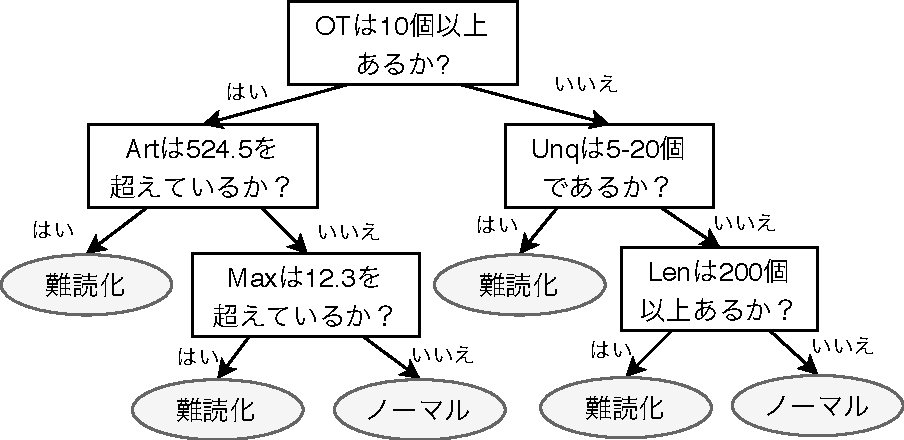
\includegraphics[width=10cm]{DT.pdf}
 \caption{決定木の例}
 \label{fig:DT}
\end{figure}

\subsubsection{分類問題}
\subsubsection*{難読化された・されていないの分類}
リサーチ・クエスチョンQ1を調べるために,難読化された・されていないプログラムの2クラスを分類するモデルを構築する.使用したアルゴリズムは,Breiman, L.によって提案された決定木を拡張したランダムフォレスト~\cite{RF}である.決定木での分類の概要は図~\ref{fig:DT}に示すように,訓練データのメトリクスをもとに,木構造の一連の質問を学習し,訓練データラベルを推測する.本実験では10本の決定木によって学習を行った.また,訓練において$P_{centos},\,P_{orig},\,P_{split}$に含まれる関数やTigressによって難読化されていない関数を難読化されていない(正),それ以外の関数は難読化された(負)というラベルを付けた.

ランダムフォレストは過学習になる可能性が高く,学習モデルの妥当性を確認するために,訓練データから除いた2割のテストデータに加えて,残りの8割を10分割交差検証でランダムフォレストによる学習を行った.10分割交差検証では,訓練データ(今回はもとデータの8割)を10個に分割し,そのうちの9個を訓練データとして学習を行い,残りの1個をテストデータとする.10個に分割されたデータそれぞれをテストデータとして10回の検証結果の平均値を推定結果として扱う.ここで,検証される指標は正解率(\textit{accuracy})である.10分割交差検証を行った後,8割の訓練データでモデルを構築し,残り2割のテストデータで最終モデルの評価を行った.学習モデルの評価結果は表~\ref{table:binclass}にまとめる.CFは10分割交差検証,Valは最終モデルの正解率を示している.適合率(\textit{precision})は予測が正と判定した中で,ラベルも正のもの,つまり,誤分類を起こさない性能の指標である.一方,再現率(\textit{recall})はラベルが正の中で,予測が正と判定したもの,つまり,正のラベルを見つけ出す能力の指標である.適合率と再現率を組みわせて評価する指標はF1スコア(\textit{F1-Score})である.正解率,適合率,再現率,F1スコアの求め方は付録~\ref{appendix:MLeval}に示す.

表~\ref{table:binclass}の10分割交差および最終モデルの検証結果より,判定モデルは妥当であり,90\%程度の正解率が得られた.このことに加えて,適合率,再現率,とF1スコアの最終モデルの性能評価指標により,難読化された・されていないの判定は可能であることが分かった.また,OPCとXRFの性能に有意差がないことが分かった.

\begin{table}[!htb]
    \caption{構築した分類モデルの評価結果}
    \begin{subtable}{.5\linewidth}
      \centering
\caption{2クラスの分類モデル}
\label{table:binclass}
\begin{tabular}[t]{cc|c|c}
\doubleRule
&  & OPC & XRF \\
\hline
\multirow{2}{*}{accuracy (\%)} & \multicolumn{1}{|c|}{CF} & 96.3 & 96.3 \\\cline{2-4}
& \multicolumn{1}{|c|}{Val} & 96.5 & 96.4 \\
\hline
\multicolumn{2}{c|}{precision (\%)} & 97 & 97 \\
\hline
\multicolumn{2}{c|}{recall (\%)} & 96 & 96 \\
\hline
\multicolumn{2}{c|}{F1-Score (\%)} & 96 & 96 \\
\bottomrule
\end{tabular}
    \end{subtable}
    \begin{subtable}{.5\linewidth}
      \centering
\caption{8クラスの分類モデル}
\label{table:allclass}
\begin{tabular}[t]{cc|c|c}
\doubleRule
&  & OPC & XRF \\
\hline
\multirow{2}{*}{accuracy (\%)} & \multicolumn{1}{|c|}{CF} & 96.2 & 96.2 \\\cline{2-4}
& \multicolumn{1}{|c|}{Val} & 96.4 & 96.4 \\
\hline
\multicolumn{2}{c|}{precision (\%)} & 97 & 97 \\
\hline
\multicolumn{2}{c|}{recall (\%)} & 96 & 96 \\
\hline
\multicolumn{2}{c|}{F1-Score (\%)} & 95 & 95 \\
\bottomrule
\end{tabular}
    \end{subtable} 
\end{table}

\subsubsection*{難読化法による分類}
リサーチ・クエスチョンQ2を調べるために,プログラムが難読化手法によって分類するモデルを構築する.訓練データにおいて$P_{centos},\,P_{orig},\,P_{split}$に含まれる関数やTigressによって難読化されていない関数をを難読化されていないというラベル$P_{norm}$,それ以外の関数はそれぞれの難読化手法によってラベルを付け,難読化法ごとに分けた8クラスを分類することを目的とする.学習アルゴリズムと妥当性の検証方法は難読化された・されていないの分類と同様に,学習モデルの全体的評価結果は表~\ref{table:allclass}に示す.適合率,再現率,F1スコアは各クラスの平均値を取ったものを示す.この表から全ての評価指標が2クラス分類と同じような結果になることが分かった.また,OPCとXRFの性能に有意差がないことが分かった.

クラス別の最終モデルの評価結果を表~\ref{table:classRes}に示す.$P_{aaa}$や$P_{vir}$のF1スコアは100\%であり,関数呼び出しおよびインタプリタエンジンを用いたの難読化方法の特徴が強く,ステルスが低いと考えられる.また,$P_{jump}$の再現率が低いことから,分岐命令をカムフラージュする難読化方法が適用された関数を見つけ出しにくく,ステルスが最も高いといえる.このことから,適用された難読化方法によって,難読化されたプログラムを分類できることが分かった.
\begin{table}[t!]
\centering
\caption{8クラス分類モデルのクラス別の評価結果}
\label{table:classRes}
\begin{tabular}[t]{c|ccc|ccc}
\doubleRule
\multirow{2}{*}{集合名称} & \multicolumn{3}{c|}{OPC} & \multicolumn{3}{c}{XRF} \\\cline{2-7}
& pre (\%) & rec (\%) & F1 (\%) & pre (\%) & rec (\%) & F1 (\%) \\
\hline
$P_{norm}$ & 96 & 100 & 98 & 96 & 100 & 98 \\
$P_{aaa}$ & 100 & 100 & 100 & 100 & 100 & 100 \\
$P_{addop}$ & 94 & 94  & 94 & 96 & 95 & 96 \\
$P_{enca}$ & 99 & 99 & 99 & 99 & 97 & 98 \\
$P_{encl}$ & 95 & 96 & 96 & 95 & 94 & 95 \\
$P_{flat}$ & 96 & 94 & 95 & 94 & 95 & 94 \\
$P_{vir}$ & 100 & 100 & 100 & 100 & 100 & 100 \\
$P_{jump}$ & 100 & 12 & 21 & 100 & 12 & 21 \\
\bottomrule
\end{tabular}
\end{table}

\newpage

\subsubsection{異常検知}
サポートベクトルマシンを拡張したOne Class SVM~\cite{OCSVM}アルゴリズムを用いて,訓練データにラベル付けなくても特徴量(メトリクス)の構造を抽出できることが学習の目的である.本実験では,放射基底関数をSVMのカーネルにし,$P_{centos},\,P_{orig},\,P_{split}$を訓練データとして扱い,モデルを構築する.構築されたモデルに評価対象プログラムを順番に与え,そのプログラムは異常(難読化されている)かどうかを予測する.

モデルの評価を行うために2クラス分類問題と同様に,難読化されたプログラムを負,難読化されていないプログラムを正のラベルを付けて正解率を評価指標とする.評価結果を表~\ref{table:ocsvmEval}に示す.訓練データの正解率の平均値は75\%以上であり,訓練データはなんらかの特徴を持つと考えられる.この表から,他のプログラム集合に比べて$P_{aaa}$や$P_{vir}$の正解率が比較的に高いことが分かった.また,OPCに比べてXRFの正解率が低いことも見られる.ただし,XRFの場合$P_{encl}$の正解率が最も高くなっており,$P_{jmp}$の正解率が上がることも確認できる.

\begin{table}[b!]
\centering
\caption{異常検知モデルの評価結果}
\label{table:ocsvmEval}
\begin{tabular}[t]{c|cc}
\doubleRule
& OPC & XRF \\
\hline
$P_{centos}$ & 87.9\% & 86.9\% \\
$P_{orig}$ & 83.8\% & 67.4\% \\
$P_{split}$ & 64.4\% & 85.7\% \\\hline
$P_{aaa}$ & 90.0\% & 80.0\% \\
$P_{addop}$ & 89.8\% & 75.7\% \\
$P_{enca}$ & 89.8\% & 78.6\% \\
$P_{encl}$ & 88.2\% & 82.1\% \\
$P_{flat}$ & 87.3\% & 79.7\% \\
$P_{vir}$ & 90.0\% & 80.0\% \\
$P_{jmp}$ & 25.0\% & 37.5\% \\
\bottomrule
\end{tabular}
\end{table}

\begin{figure}[bhtp]
  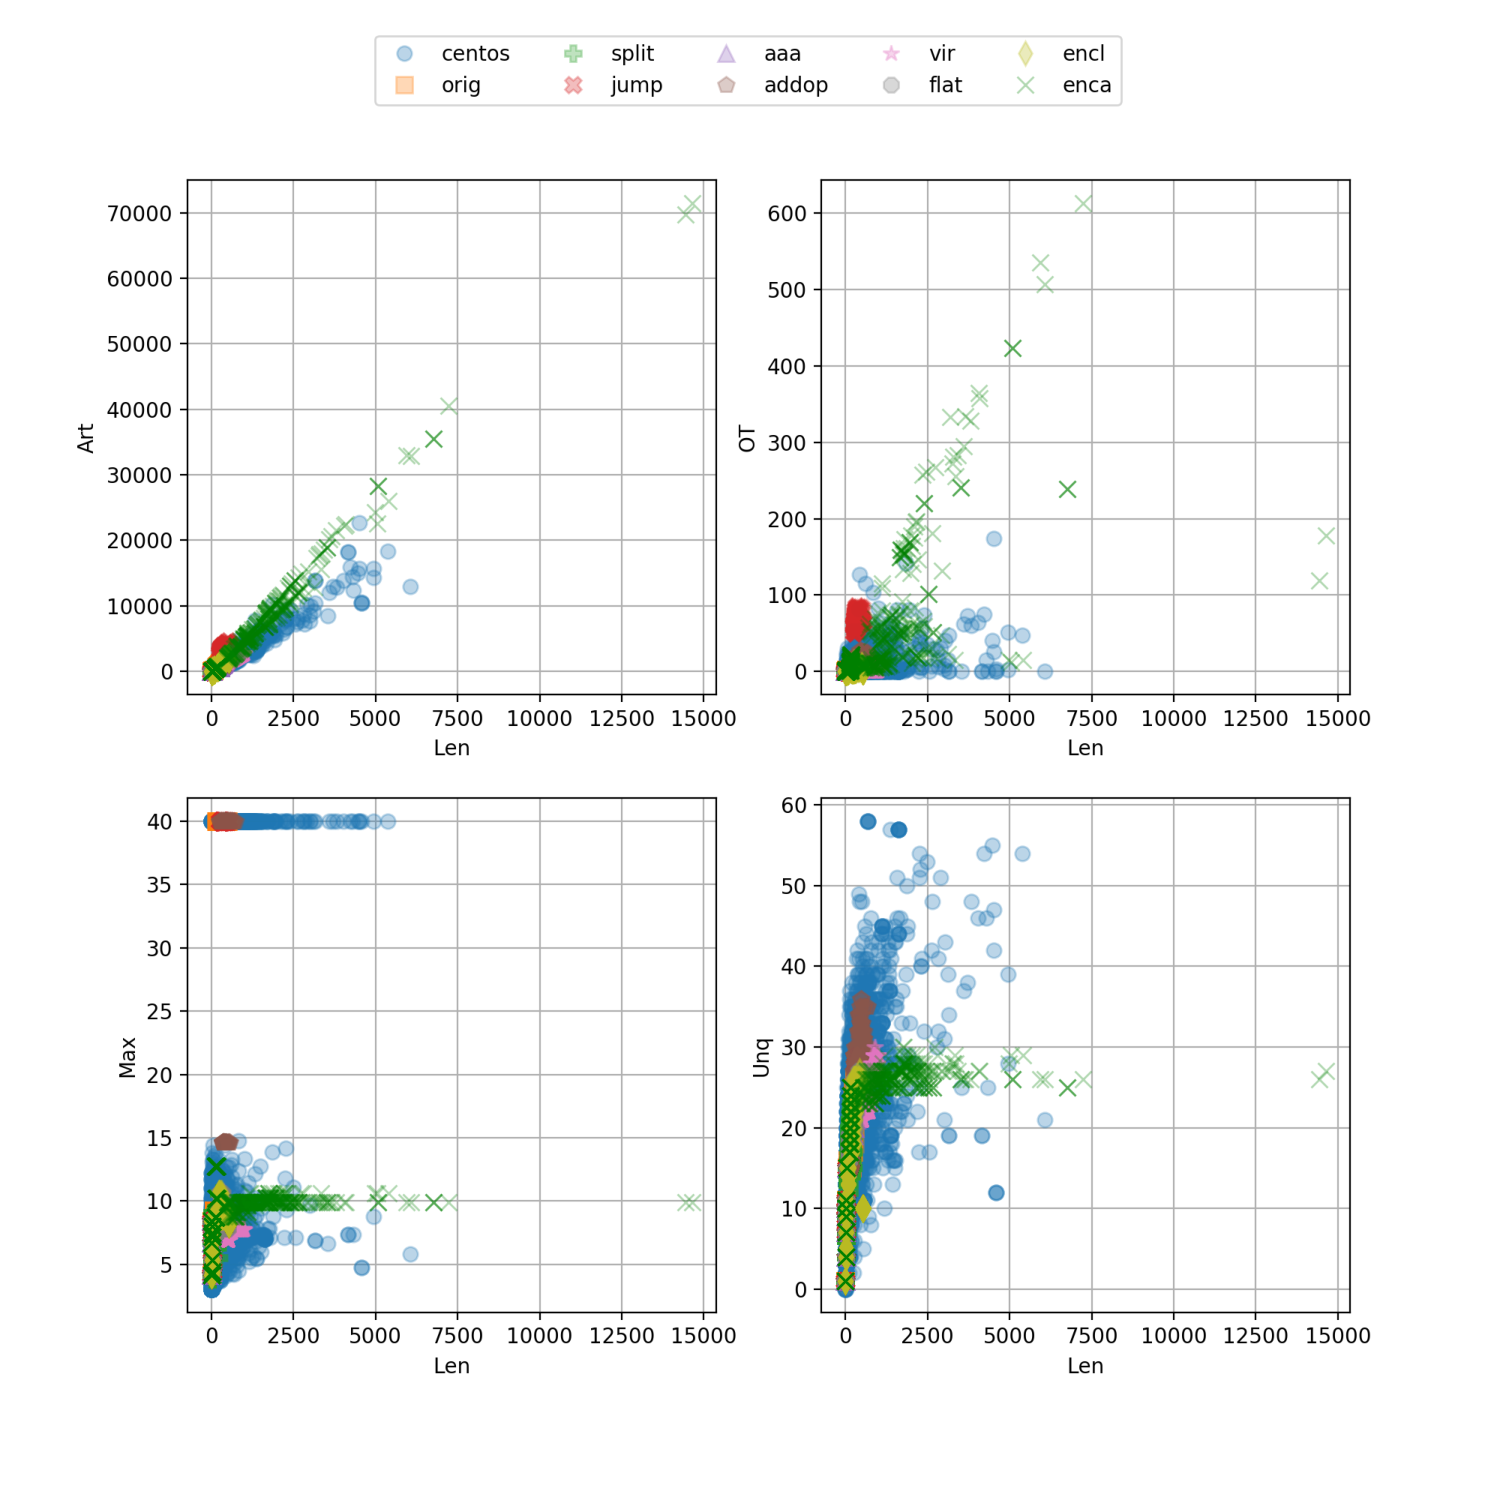
\includegraphics[width=17cm]{opc_OCSVM_all_b4.pdf}
  \caption{検出前}
  \label{fig:OCSVM_b4}
\end{figure}

\begin{figure}[bhtp]
  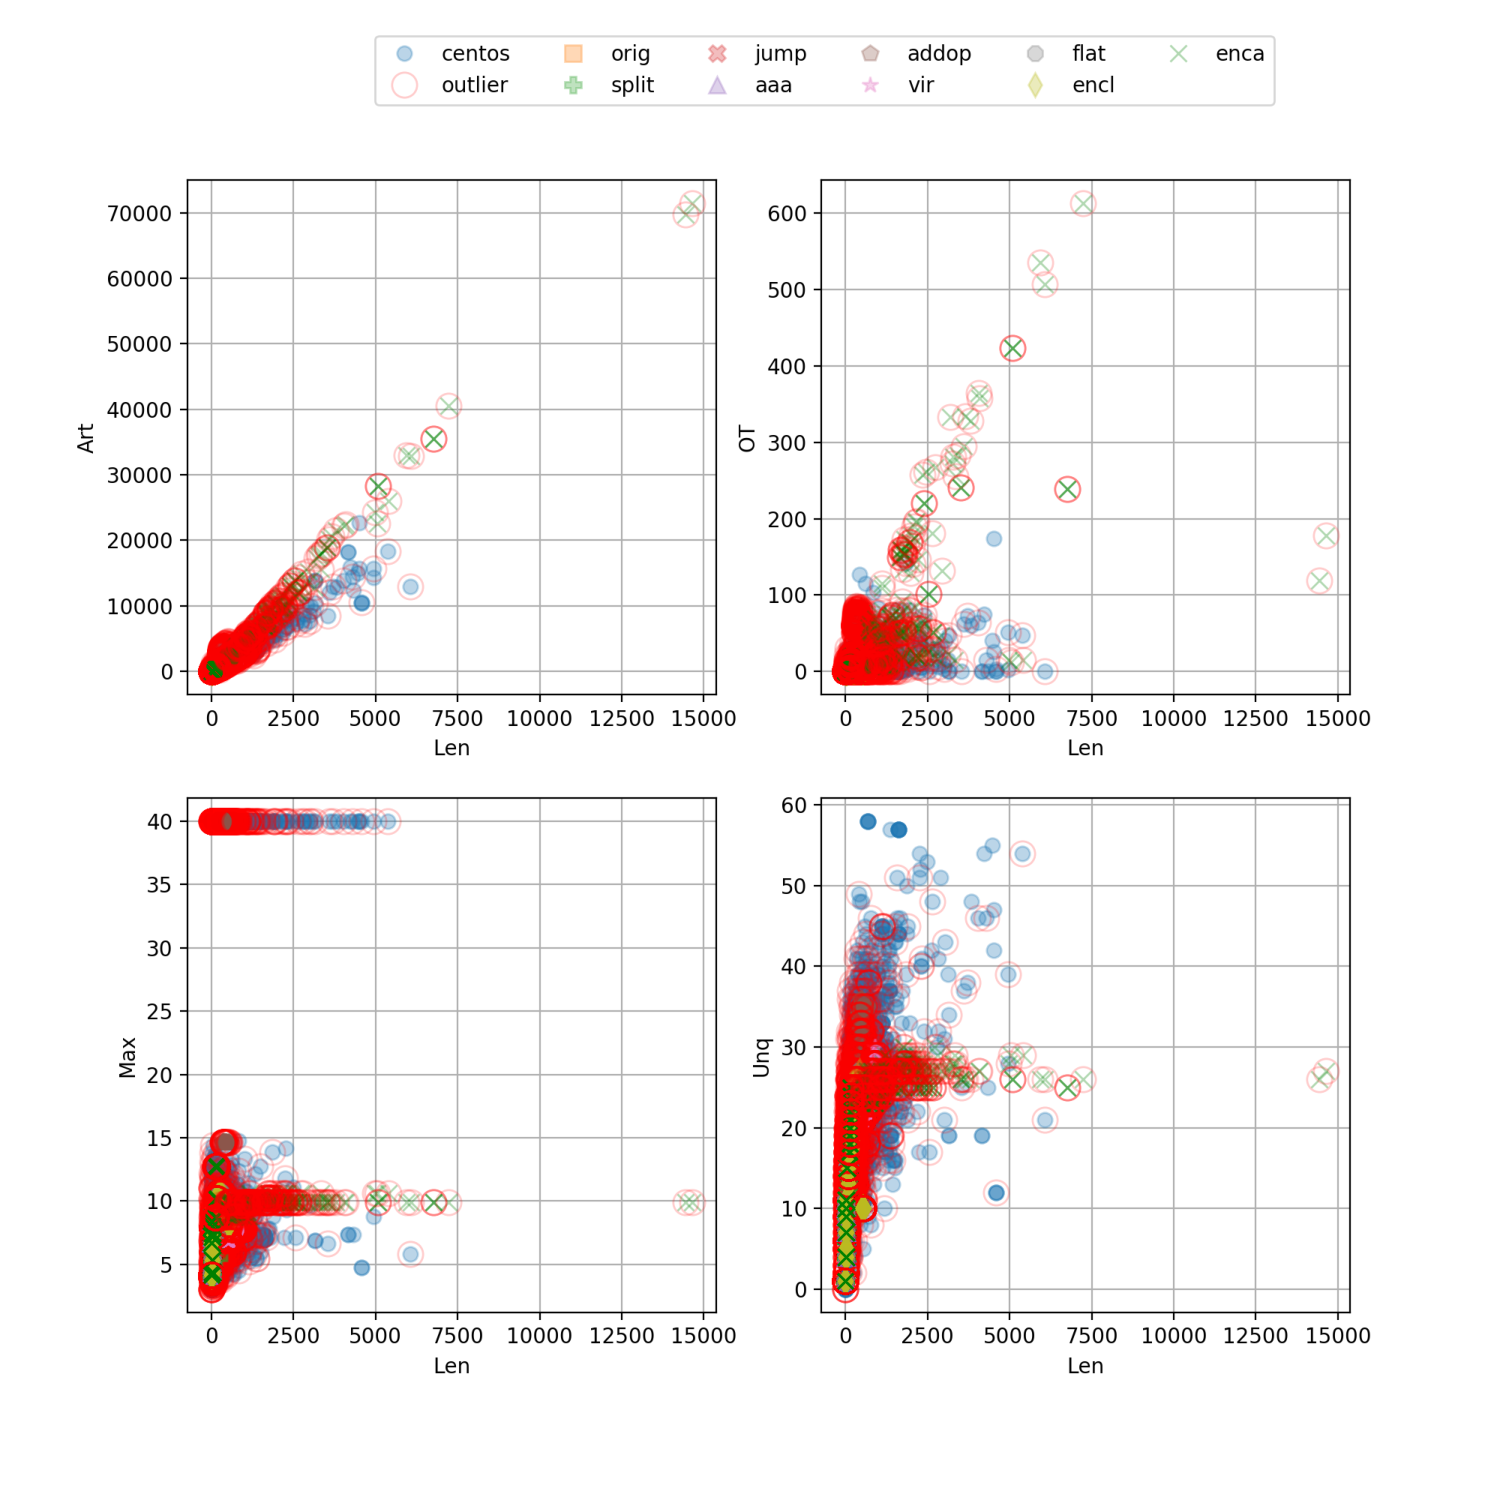
\includegraphics[width=17cm]{opc_OCSVM_all.pdf}
  \caption{検出後}
  \label{fig:OCSVM_af}
\end{figure}

OPCの異常検知前後を図~\ref{fig:OCSVM_b4}と図~\ref{fig:OCSVM_af}に示している.横軸はLen,縦軸は左上の図から順に右へ順にArt, OT, Max, Unqを示して,同じコード変形が適用された関数が同じ座標にある場合,色の濃さによって見分けられるようにした.異常として検出された箇所は赤い塗り潰されていない円形で囲まれている.図~\ref{fig:OCSVM_b4}を見ると,$P_{enca}$「\ding{53}」が$P_{norm}$「青い円形」よりもLenが大きく,これが整数の算術の難読化特徴であると考えらる.また,図~\ref{fig:OCSVM_b4}のLenとOTの関係図を見ると,$P_{jmp}$「\ding{54}」は,他のプログラム集合に比べて傾きが異なっていることが分かった.

異常検知を行なった後の図~\ref{fig:OCSVM_af}を見ると,いくつかの誤認したところを確認できる.この異常検知モデルにより,各難読化手法は特徴を持つことを確認できるが,訓練データにラベルを付けないため,分類モデルに比べて正解率が低くなると考えられる.

\subsection{ステルス数値化法の有効性}
ランダムフォレストのモデル構築に当たって,特徴量の重要度を計算することもできる.特徴量の重要度は以下の手順に従って求められる.

\begin{enumerate}[label=\arabic*.]
  \item ある特徴量に属するデータをランダムに変化させ,変化前後の正解率の差を求める.
  \item 特徴量の数だけ手順1を繰り返す.本研究では,特徴量が5つあるため,手順1を5回繰り返す.
  \item 正解率の差を基準に,特徴量を順に並べ替える.正解率の差が大きいほどその特徴量が重要である.
\end{enumerate}

分類モデルにおけるOPCの特徴量の重要度を図~\ref{fig:featureImportance}に示す.ここではXRFの図を表示しないが,OTが最も重要であることが分かる.~\ref{sub:metrics}章で説明したように,OTは定められた驚き値の閾値を超えたコード片の総数であることから,驚き値は有効なステルス数値化法といえる.

\begin{figure}[!h]
\centering
\begin{tikzpicture}
\begin{axis}[
legend pos=outer north east,
xbar, xmin=0, xmax=40,
xmajorgrids=true,
xlabel={重要度 (\%)},ylabel={特徴量},
symbolic y coords={Len, Max, Art, Unq, OT},
ytick=data,
nodes near coords, 
nodes near coords align={horizontal},
ytick=data,
]
\addplot coordinates {(30.72,OT) (12.1,Max) (21.03,Art) (25.55,Unq) (10.61,Len)};
\addplot coordinates {(31.86,OT) (9.77,Max) (24.66,Art) (21.1,Unq) (12.63,Len)};
\legend{2クラス,8クラス}
\end{axis}
\end{tikzpicture}
\caption{特徴量の重要度}
\label{fig:featureImportance}
\end{figure}

\newpage

\section{まとめ}  \label{sec:concl}
本研究では,機械学習によってプログラムが難読化されているかどうかを判定するフレームワークを提案した.ケーススタディではフレームワークの有用性を調べるために,合計3,052のプログラムを用いてステルスを評価する機械学習のモデルを構築した.最良のモデルでは95\%以上の精度でデータセットにあるプログラムを判定でき,難読化された・されていないプログラムは分類できることが分かる.各難読化手法には特徴があり,分岐命令をカムフラージュする難読化方法の特徴が,実験で適用した他の難読化手法よりも弱く,ステルスが高いと考えられる.

今後の課題として,難読化方法やメトリクスの種類を増やすことで,さらに有用なステルス評価モデルを検討することが挙げられる.また,ステルス評価の学習モデルを用いて,複数の難読化方法を組み合わせることによってステルスの高いプログラムを生成する難読化システムの開発も研究テーマとして考えられる.

\newpage

\renewcommand{\refname}{参考文献・参考URL}
\begin{thebibliography}{9}
\addcontentsline{toc}{section}{参考文献}% 目次に加える
\bibitem{resilience-banescu}
Banescu, S., Collberg, C., Pretschner, A.
``Predicting the Resilience of Obfuscated Code Against Symbolic Execution Attacks via Machine Learning'',
In \textit{Proc. of the 26th USENIX Security Symposium} (2017), USENIX, pp.661-678

\bibitem{pinpoint}
Kanzaki, Y., Thomborson, C., Monden, A., and Collberg, C.
``Pinpointing and Hiding Suprising Fragments in an Obfuscated Program'',
In \textit{Proc. of the 5th Program Protection and Reverse Engineering Workshop} (2015), PPREW-5, ACM, pp.8:1-8:9.

\bibitem{code-art}
Kanzaki, Y., Monden, A., and Collberg, C.
``Code Artificiality: A Metric for the Code Stealth Based on an N-gram Model'',
In \textit{Proc. of the 1st International Workshop on Software Protection} (2015), IEEE Press, pp.31-37

\bibitem{tigress}
Collberg, C.: The Tigress C Diversifier/Obfuscator,
\url{http://tigress.cs.arizona.edu/}. (accessed: Feb. 2018)

\bibitem{jmp-obf}
村上隼之助,神崎雄一郎,門田暁人, 
``分岐命令のカムフラージュに基づくプログラムの制御フローの隠ぺい'',
火の国情報シンポジウム2018,情報処理学会九州支部 (2018).

\bibitem{movfuscator}
Domas, C.: M/o/Vfuscator2 :: the single instruction C compiler,
\url{https://github.com/xoreaxeaxeax/movfuscator}.

\bibitem{pearson}
Pearson, K.
``Note on regression and inheritance in the case of two parents'',
\textit{Proc. of the Royal Society of London 58} (1895), 240-242

\bibitem{RF}
Breiman, L.
``Random forests'',
\textit{Machine Learning 45} (2001), 5-32

\bibitem{OCSVM}
Sch\"{o}lkopf, B., Platt, J. C., Shawe-Taylor, J., Smola, A. J., Williamson, R. C.
``Estimating the Support of a High-Dimensional Distribution'',
\textit{Neural computation 13.7} (2001), 1443-1471
\end{thebibliography}
\noindent (URLは2018年2月現在)

\newpage
\section*{謝辞}
\addcontentsline{toc}{section}{謝辞}% 目次に加える

本研究を行うにあたり,ご指導を頂いた卒業研究指導教員の神崎雄一郎准教授に心より感謝致します.日常の議論を通じて多くの知識を頂き,本当にありがとうございます.


\newpage
%付録

\begin{appendices}
%\appendix
%\def\thesection{\ \ \ 付録\Alph{section}}
\section{コードの不自然さと驚き値}  \label{appendix:artAndsurp}
本論文では,ソフトウエアを構成するプログラムの一部あるいは全部をx86アーキテクチャのアセンブリ言語で表したものをコードと呼ぶ.また,コードに含まれている1つのアセンブリ命令をN個ずつ並べたものをN-gramといい,例えばコードが\texttt{mov},\texttt{and},\texttt{push},\texttt{push},から構成されているとき,3つずつ並べると,「\texttt{mov-and-push}」,「\texttt{and-push-push}」という2つの命令列を得て,コードを3-gramに分割したという.コードのN-gramは長さNのコード片とも呼び,$i_j^n$はコード全体の$j$番目から始まる長さ$n$のコード片を示し,1つの命令の場合は,単に$i_j$と記述する.

N-gramモデルに基いたコードの不自然さの数値化法~\cite{code-art}と同様に,難読化されていないプログラムのコードを多く集めたものをコーパスとした確率的言語モデルを用いて,与えられた命令列の自然さを求める.具体的な例として,コードの全体$C$が$m$個の命令から構成され,$i_1^m=i_1i_2...i_m$の命令列で表したとき,生起確率$P(i_1^m)$は次のように近似する.
\begin{equation}
  P(i_1^m)\approx\prod_{k=1}^m P(i_k|i_{k-N+1}^{k-1})
\end{equation}
生起確率$P(i_1^m)$の値が大きいほど命令列が自然であると考えられる.この生起確率$P(i_1^m)$から底が2の対数を取って得られた値は,コード全体の不自然さをビット単位で表したものであり,次のように定義する.
\begin{equation}
  Artificiality\quad A(C)=-log_2P(i_1^m)\,\quad[bit]
\end{equation}
式(1)とは逆であり,$A(C)$が大きいほどコード$C$が不自然であると考える.

一方,目立つコード片はコーパスに出現する数が最も少なく,コード片の目立つさの度合「驚き値」(\textit{Surprisal})は次のような式で定義される.
\begin{equation}
  S(i_j^n)=-log_2P(i_{j+n-1}|i_j^{n-1})\quad[bit]
\end{equation}
例えば,上記の3-gramを考えると,後者の驚き値は$S(i_2^3)=S$(\texttt{and-push-push})と示し,実際本研究で使用したコーパスでは4.365と計算される.不自然さと同様に$S()$が大きいほどコーパスに出現する数が少なく,本研究では,コーパスに出現しないコード片を無限大でない大きい値を与える.


\newpage

%\def\thesection{\ \ \ 付録\Alph{section}}

\section{\texttt{RandomFuns}のパラメータ} \label{appendix:randfuns}
\begin{description}
  \item[\texttt{RandomFunsControlStructures}]\hfill\break
  生成される関数の制御構造を定められた文法記述によって調整する.本実験では「\texttt{(if (bb n)(bb n)}」,「\texttt{(for (bb n))}」,「\texttt{(if (bb n) (for (bb n)))}」の3つの中から構造を選ぶものとする.文法にある\texttt{(bb n)}は基本ブロックに\texttt{n}個のステートメントを生成する.なお,\texttt{n}は\texttt{RandomFunsBasicBlockSize}によって調整でき,今回は,$n\in$ \{1,2\},の2つの中から選ぶものとする.
  \item[\texttt{RandomFunsType}]\hfill\break
  入出力とステートメント配列のデータ型を調整する.今回は,Type $\in$ \{char, short, int, long\},の4つの中から選ぶものとする.
  \item[\texttt{RandomFunsForBound}]\hfill\break
  生成されたプログラムにある\texttt{for}文の範囲を調整する.今回は,Bound $\in$ \{constant, boundedInput, boundedAny\},の3つの中から選ぶものとする.なお,constantは整数のリテラルを用い,boundedInputとboundedAnyは範囲外の添字を選択しないようし,それぞれ入力配列からの値と,任意のソースからの値を用いて\texttt{for}文の範囲を決定する.
  \item[\texttt{RandomFunsOperators}]\hfill\break
  生成された関数内に使用可能なオペレータを設定する.本実験では,Opr $\in$ \{簡単な比較と算術演算子,複雑な比較と算術演算子,比較とビット演算子,全ての演算子 \},の4つの中から選ぶものとする.
  \item[\texttt{RandomFunsPassword}]\hfill\break
  ユーザが標準入力から入力するパスワードを設定する.本実験では,「\texttt{secret}」と設定し,\texttt{RandomFunsPasswordCheckCount}を1に設定することでパスワード確認を1回行う.
  \item[\texttt{RandomFunsFailureKind}]\hfill\break
  上記のパスワード確認,有効期限確認,実行許可コードが失敗した場合,「\texttt{abort()}」という関数が呼び出される.
  \item[\texttt{RandomFunsTimeCheckCount}]\hfill\break
  ライセンスチェックのような有効期限の確認ルーチンを挿入する.今回は,1と設定した.ただし,動作確認のため有効期限確認を常に成功(有効期限内)にしている.
  \item[\texttt{RandomFunsActivationCodeCheckCount}]\hfill\break
  生成されたプログラムの実行許可コードの確認回数を設定する.今回は,1と設定した.
  \item[\texttt{RandomFunsPointTest}]\hfill\break
  設定された値と,生成された関数によって変換された入力が一致した場合``You win!''のメッセージを標準出力する.今回は,実行時に4つのコマンドラインの引数が42
  である場合メッセージを出力するように設定した.
\end{description}
したがって,合計の組み合わせの数が$3\times2\times4\times3\times4=288$個のプログラムである.なお,生成のシードを7にし,上記以外のパラメータをデフォルト値に設定した.


\section{正解率,適合率,再現率,とF1スコア} \label{appendix:MLeval}
あるクラス$C_i$に対する分割表を表~\ref{table:confmat}に示している.

\begin{table}[thb!]
\centering
\caption{分割表}
\label{table:confmat}
\begin{tabular}[t]{c|cc}
\doubleRule
& 実際に$C_i$に属する & 実際に$C_i$に属さない \\
\hline
$C_i$と判定される & \textit{true positive (tp)} & \textit{false positive (fp)} \\
$C_i$以外と判定される & \textit{false negative (fn)} & \textit{true negative (tn)} \\
\bottomrule
\end{tabular}
\end{table}

この表に従って,正解率,適合率,再現率,およびF1スコアは次式によって求めらる.
\begin{equation} \label{eq:acc}正解率=\frac{正解の判定}{全てのサンプル}=\frac{tp+tn}{tp+tn+fp+fn} \end{equation}
\begin{equation}適合率=\frac{正しくC_iに属すると判定される}{C_iと判定される}=\frac{tp}{tp+fp} \end{equation}
\begin{equation}適合率=\frac{正しくC_iに属すると判定される}{実際にC_iに属する}=\frac{tp}{tp+fn} \end{equation}
\begin{equation}\label{eq:f1}F1スコア=2\times\frac{適合率\times{再現率}}{適合率+再現率} \end{equation}
式(\ref{eq:acc})の正解率は,正しい判定の割合を示す.また,式(\ref{eq:f1})より,適合率又は再現率が0である場合,F1スコアが0になることが確認できる.再現率と適合率の両方が0である場合,テストデータに偏りがある($C_i$に属する項目がない等)と考えられ,テストデータは無効であると考えられる.

\end{appendices}
\end{document}
